 \mode*
\mode<all>{\topsection{Geometria hiperboliczna}}
\begin{frame}[<+->]
W ujęciu tradycyjnym, nazywanym geometrią syntetyczną, geometria euklidesowa przedstawiana jest jako system aksjomatyczny, w którym wszystkie twierdzenia muszą wynikać z aksjomatów, czyli zdań przyjmowanych z góry jako prawdziwe.
\end{frame}
%%%%%%next-slide%%%%%

\mode<all>{\midsection{Aksjomaty Euklidesa}}
%%%%%%next-slide%%%%%
\begin{frame}[<+->]

W podanym przez siebie systemie Euklides wyróżnił pięć aksjomatów płaszczyzny nazywanej później również euklidesową:
\begin{enumerate}
\item Dowolne dwa punkty można połączyć odcinkiem.
\item Dowolny odcinek można przedłużyć nieograniczenie (uzyskując prostą).
\item Dla danego odcinka można zaznaczyć okrąg o środku w jednym z jego końcowych punktów i promieniu równym jego długości.
\item Wszystkie kąty proste są przystające.
\item Dwie proste, które przecinają trzecią w taki sposób, że suma kątów wewnętrznych po jednej stronie jest mniejsza od dwóch kątów prostych, przetną się z tej właśnie strony.
\end{enumerate}
\end{frame}
%%%%%%next-slide%%%%%

Ponieważ piąty postulat wzbudzał wiele podejrzliwości (już chociażby przez swoją długość) każdy szanujący się matematyk w pomiędzy V-XVIIw. musiał podjąć się próby udowodnienia go jako twierdzenia wynikającego z pozostałych czterech. W XIXw. okazało się jednak, że piąty postulat jest niezależny od pozostałych czterech i na tej podstawie zostały sformułowane różne geometrie: system aksjomatyczny przyjmujący piąty postulat nazywamy \textbf{geometrią euklidesową}, zaś system przyjmujący \textit{zaprzeczenie} piątego postulatu nazywany jest obecnie \textbf{geometrią hiperboliczną}.


%%%%%%next-slide%%%%%
\begin{frame}[<+->]
Przez wieki prób dowodzenia powstało wiele innych twierdzeń \textit{równoważnych} z piątym aksjomatem, np.
\begin{description}
\item [Playfair] Przez dany punkt można poprowadzić dokładnie jedną prostą równoległą do danej prostej.
\item [\textbullet]Dla każdej prostej i każdego punktu poza nią istnieje dokładnie jedna prosta równoległa do niej przechodząca przez ten punkt.
\item [\textbullet]Jeśli trzy kąty w czworokącie są proste, to i czwarty jest prosty.
\item [\textbullet]Istnieje prostokąt.
\item [\textbullet]Twierdzenie Pitagorasa.
\item [W. Bolyai] Na każdym trójkącie można opisać okrąg.
\end{description}
\end{frame}
\begin{frame}
\begin{description}
\item [J. Wallis] Istnieją dwa trójkąty podobne, ale nieprzystające.
\pause\item [\textbullet]Jeśli dwie proste są równoległe do trzeciej, to są również między sobą równoległe.
\pause\item [\textbullet]Istnieje trójkąt o sumie kątów wewnętrznych równej $\pi$.
\pause\item [\textbullet]Suma kątów wewnętrznych w każdym trójkącie jest taka sama.
\pause\item [Aksjomat trójkąta] Suma kątów wewnętrznych w każdym trójkącie wynosi $\pi$.
\end{description}
\mode<presentation>{\pause Jaki wniosek można wyprowadzić z aksjomatu trójkąta i twierdzenia Gaussa-Bonneta?}

\end{frame}
Zwłaszcza to ostatnie stwierdzenie powinno nas zaciekawić w kontekście niedawno rozważanego lokalnego twierdzenia Gaussa-Bonneta. Wnioskiem z niego będzie zerowa krzywizna całej powierzchni będącej modelem geometrii euklidesowej (tj. na której postulaty Euklidesa są spełnione).


%%%%%%next-slide%%%%%
\mode<all>{\midsection{Definicja płaszczyzny hiperbolicznej I}}
W sposób aksjomatyczny płaszczyznę hiperboliczną można zdefiniować analogicznie jak płaszczyznę euklidesową.
\begin{frame}
\begin{definicja}
\textbf{Płaszczyzną hiperboliczną} nazywamy dowolny zbiór $\mathcal{P}$ wraz z rodziną podzbiorów zwanych prostymi i odległością geometryczną spełniający \textit{pierwsze cztery} aksjomaty Euklidesa, oraz następujący \textbf{hiperboliczny aksjomat} o równoległych:
\begin{itemize}
\pause \item [5'.] Dla pewnej prostej $\mathcal{D}\subset \mathcal{P}$ i pewnego punktu $M\in \mathcal{P}$ nieleżącego na $\mathcal{D}$ istnieją co najmniej dwie różne proste $\Delta_1$, $\Delta_2$ przechodzące przez $M$ i rozłączne z $\mathcal{D}$.
\end{itemize}
\end{definicja}
\pause 
\begin{uwaga}
Wszystkie własności płaszczyzny euklidesowej, które można udowodnić nie posługując się aksjomatem Euklidesa o równoległych (są to tzw. twierdzenia \textbf{geometrii absolutnej}), przysługują również płaszczyźnie hiperbolicznej.
\end{uwaga}

\end{frame}
%%%%%%next-slide%%%%%

Układ aksjomatyczny ma sens tylko w takiej sytuacji, gdy jest niesprzeczny. 
W następnym paragrafie zbudujemy model arytmetyczny płaszczyzny hiperbolicznej, analogiczny do modelu
kartezjańskiego płaszczyzny euklidesowej. 

\mode<all>{\midsection{Model Poincar\'{e}go}}
\begin{frame}
Pierwszy model geometrii hiperbolicznej został zaproponowany przez H. Poincar\'{e}go w roku 1882 i nazywany jest 
\textbf{modelem Poincar\'{e}go} płaszczyzny hiperbolicznej na górnej półpłaszczyźnie.

\pause\begin{definicja} 
\textbf{Górną półpłaszczyzną} lub \textbf{półpłaszczyzną Poincar\'{e}go}
nazywamy zbiór \[\mathcal{H}\define\{\,(x,y)\in \R^2\mid y>0\,\}.\]
\pause \textbf{Prostą hiperboliczną} w $\mathcal{H}$ nazywamy każdy podzbiór 
$\mathcal{D}\subset \mathcal{H}$ określony równaniem postaci: 
\begin{align*}
x=&x_{0}, & \text{albo} & & r^2&=(x-x_{0})^{2}+y^{2},
\end{align*}gdzie $x_{0}$ i $r>0$ są dowolnymi stałymi.
\end{definicja}

\end{frame}

\mode<all>{\midsection{Geometria elementarna na półpłaszczyźnie Poincar\'ego}}
\begin{frame}
Proste hiperboliczne na półpłaszczyźnie Poincar\'{e}go są to półproste otwarte na górnej płaszczyźnie 
$\R^2$ mające początki na osi $x$ i prostopadłe do tej osi albo półokręgi otwarte oparte na osi $x$.

\begin{center}

\usetikzlibrary{arrows}

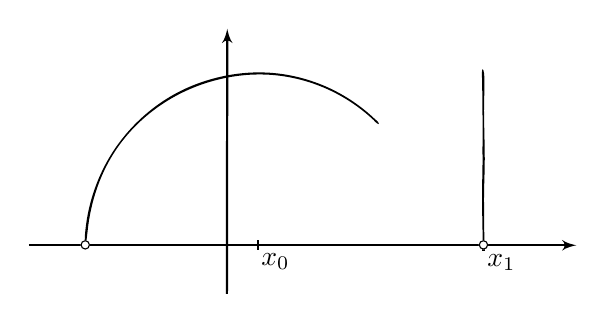
\begin{tikzpicture}[y=0.80pt, x=0.8pt,yscale=-1,scale=0.3, inner sep=0pt, outer sep=0pt]
\begin{scope}[shift={(220.0315,-356.64289)}]% layer1
  \begin{scope}[shift={(3147.7678,-1427.0496)}]% g1988
    % path2584-0-9
    \path[draw=black,line join=miter,line cap=butt,line width=0.800pt,-latex']
      (-3367.7993,2109.6489) -- (-2543.3619,2109.6489);

    % path2582-4-4
    \path[draw=black,line join=miter,line cap=butt,line width=0.800pt,-latex']
      (-3069.5306,2182.6982) -- (-3068.9608,1783.6932);

  \end{scope}
  
  \path[cm={{1.0,0.0,0.0,-1.0,(3140.5045,2591.4389)}},color=black,fill=black,line
    width=0.800pt] (-3275.9219,1924.7961) .. controls (-3274.0064,1949.1681) and
    (-3268.7857,1973.2307) .. (-3260.4507,1996.1851) .. controls
    (-3252.1157,2019.1395) and (-3240.6585,2040.9822) .. (-3226.3161,2060.7308) ..
    controls (-3218.1656,2071.9535) and (-3209.1713,2082.5585) ..
    (-3199.3587,2092.3795) .. controls (-3187.1384,2104.6086) and
    (-3173.7246,2115.6571) .. (-3159.3392,2125.2681) .. controls
    (-3144.9538,2134.8790) and (-3129.5957,2143.0509) .. (-3113.5346,2149.5012) ..
    controls (-3113.5346,2149.5012) and (-3113.5346,2149.5012) ..
    (-3113.5346,2149.5012) .. controls (-3113.1699,2149.6476) and
    (-3112.8048,2149.7932) .. (-3112.4394,2149.9379) .. controls
    (-3097.0993,2156.0119) and (-3081.2310,2160.7397) .. (-3065.0449,2163.9877) ..
    controls (-3048.8588,2167.2358) and (-3032.3546,2169.0015) ..
    (-3015.8188,2169.1274) .. controls (-2999.8796,2169.2486) and
    (-2983.9164,2167.8441) .. (-2968.2563,2164.8673) .. controls
    (-2951.0237,2161.5916) and (-2934.1341,2156.5782) .. (-2917.9460,2149.8888) ..
    controls (-2888.8995,2137.8841) and (-2862.1914,2120.4577) ..
    (-2839.4920,2098.9265) .. controls (-2836.8258,2096.8474) and
    (-2835.1135,2095.0508) .. (-2834.1618,2093.7239) .. controls
    (-2833.2100,2092.3970) and (-2833.0168,2091.5377) .. (-2833.3988,2091.2677) ..
    controls (-2833.7809,2090.9978) and (-2834.7367,2091.3147) ..
    (-2836.1176,2092.3096) .. controls (-2837.4985,2093.3041) and
    (-2839.3032,2094.9740) .. (-2841.4364,2097.4050) .. controls
    (-2863.9308,2118.5347) and (-2890.3362,2135.6017) .. (-2918.9853,2147.3259) ..
    controls (-2934.7322,2153.7707) and (-2951.1412,2158.6130) ..
    (-2967.8722,2161.7989) .. controls (-2983.6622,2164.8057) and
    (-2999.7601,2166.1917) .. (-3015.8188,2166.0130) .. controls
    (-3031.7764,2165.8355) and (-3047.6958,2164.1152) .. (-3063.3128,2161.0052) ..
    controls (-3078.9298,2157.8952) and (-3094.2448,2153.3978) ..
    (-3109.0654,2147.6431) .. controls (-3110.1330,2147.2286) and
    (-3111.2004,2146.8062) .. (-3112.2672,2146.3759) .. controls
    (-3127.6217,2140.1844) and (-3142.8538,2132.3217) .. (-3157.2876,2122.9313) ..
    controls (-3171.7213,2113.5409) and (-3185.3479,2102.6268) ..
    (-3197.5901,2090.6108) .. controls (-3207.7492,2080.6412) and
    (-3216.9054,2069.8903) .. (-3224.9220,2058.7675) .. controls
    (-3231.9232,2049.0535) and (-3237.9985,2039.0203) .. (-3243.2902,2028.7549) ..
    controls (-3248.5820,2018.4895) and (-3253.0914,2007.9901) ..
    (-3256.9204,1997.2658) .. controls (-3260.7494,1986.5415) and
    (-3263.8991,1975.5911) .. (-3266.4128,1964.3674) .. controls
    (-3268.9264,1953.1438) and (-3270.8056,1941.6460) .. (-3272.0133,1929.7871) ..
    controls (-3272.2533,1927.6235) and (-3272.5773,1924.8845) ..
    (-3272.9079,1922.1027) .. controls (-3273.2386,1919.3208) and
    (-3273.5755,1916.4957) .. (-3273.9090,1914.1696) .. controls
    (-3274.2424,1911.8435) and (-3274.5767,1910.0163) .. (-3274.9407,1909.2419) ..
    controls (-3275.3047,1908.4675) and (-3275.7077,1908.7460) ..
    (-3276.1132,1910.6445) .. controls (-3276.5112,1914.8042) and
    (-3276.2471,1920.1155) .. (-3275.9219,1924.7961) -- cycle;
\filldraw[white](-135,682) circle (5pt);
  \draw(-135,682) circle (5pt);
  % path2032
  \path[draw=black,line join=miter,line cap=butt,line width=0.800pt]
    (124.5441,675.1125) -- (124.5441,689.1781);

  % text2036
  \path[fill=black] (130.17809,718.74866) node[above right] (text2036) {$x_0$};

  \begin{scope}[shift={(2906.3668,-1422.8206)}]% g1992
  \end{scope}
  % path2040
  \path[fill=black] (462.1640,424.4330) .. controls (462.8869,445.4724) and
    (462.7591,466.5429) .. (463.0949,487.6326) .. controls (463.4306,508.7221) and
    (462.9294,529.8297) .. (463.1058,550.9405) .. controls (463.2821,572.0514) and
    (462.1360,593.1655) .. (462.3806,614.2687) .. controls (462.6252,635.3717) and
    (462.9609,656.4639) .. (463.5014,677.5303) .. controls (462.3453,683.3565) and
    (467.2841,682.9759) .. (465.9389,677.3598) .. controls (465.5684,656.4858) and
    (465.4085,635.5856) .. (465.3263,614.6761) .. controls (465.2441,593.7667) and
    (466.5393,572.8483) .. (466.4796,551.9380) .. controls (466.4199,531.0278) and
    (465.6750,508.1669) .. (465.3719,487.2905) .. controls (465.0687,466.4141) and
    (466.5077,447.5234) .. (465.6953,426.7155) .. controls (465.4684,422.9163) and
    (464.1545,415.0762) .. (462.4766,418.3411) .. controls (462.0479,420.1309) and
    (462.1372,422.4139) .. (462.1640,424.4330) -- cycle;
  % path2032-8
  \path[draw=black,line join=miter,line cap=butt,line width=0.800pt]
    (464.6885,677.6608) -- (464.6885,691.7264);
\filldraw[white](464.5,682) circle (5pt);
  \draw(464.5,682) circle (5pt);

  % text2036-5
  \path[fill=black] (470.32239,721.29706) node[above right] (text2036-5) {$x_1$};

\end{scope}

\end{tikzpicture}


Półproste hiperboliczne.
\end{center}

\end{frame}
\begin{frame}
\begin{center}

\usetikzlibrary{arrows}

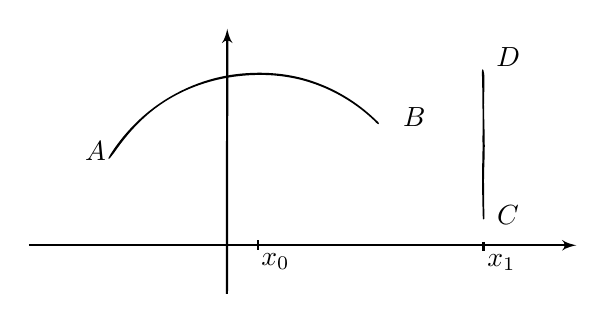
\begin{tikzpicture}[y=0.80pt, x=0.8pt,yscale=-1,scale=0.3, inner sep=0pt, outer sep=0pt]
\begin{scope}[shift={(220.0315,-356.64289)}]% layer1
  \begin{scope}[shift={(3147.7678,-1427.0496)}]% g1988
    % path2584-0-9
    \path[draw=black,line join=miter,line cap=butt,line width=0.800pt,-latex']
      (-3367.7993,2109.6489) -- (-2543.3619,2109.6489);

    % path2582-4-4
    \path[draw=black,line join=miter,line cap=butt,line width=0.800pt,-latex']
      (-3069.5306,2182.6982) -- (-3068.9608,1783.6932);

  \end{scope}
  % path2010
  \path[cm={{1.0,0.0,0.0,-1.0,(3140.5045,2591.4389)}},color=black,fill=black,line
    width=0.800pt] (-3235.0518,2049.7501) .. controls (-3224.7011,2065.1961) and
    (-3212.8770,2079.6329) .. (-3199.6736,2092.6944) .. controls
    (-3185.8590,2106.3606) and (-3170.5392,2118.5216) .. (-3154.0121,2128.7327) ..
    controls (-3141.0975,2136.7119) and (-3127.5595,2143.6755) ..
    (-3113.5002,2149.4165) .. controls (-3092.3728,2158.0428) and
    (-3070.0886,2163.9194) .. (-3047.4083,2166.5846) .. controls
    (-3036.9248,2167.8165) and (-3026.3793,2168.5155) .. (-3015.8188,2168.6123) ..
    controls (-3002.0742,2168.7382) and (-2988.3043,2167.8430) ..
    (-2974.6857,2165.8204) .. controls (-2961.0670,2163.7979) and
    (-2947.6000,2160.6459) .. (-2934.5389,2156.2799) .. controls
    (-2928.9138,2154.3996) and (-2923.3554,2152.3245) .. (-2917.8777,2150.0571) ..
    controls (-2888.1454,2137.7477) and (-2860.8772,2119.7384) ..
    (-2837.9127,2097.4492) .. controls (-2835.8085,2095.8616) and
    (-2834.4951,2094.4459) .. (-2833.8004,2093.3682) .. controls
    (-2833.1057,2092.2905) and (-2833.0283,2091.5492) .. (-2833.3979,2091.2668) ..
    controls (-2833.7675,2090.9844) and (-2834.5829,2091.1593) ..
    (-2835.6950,2091.8948) .. controls (-2836.8072,2092.6302) and
    (-2838.2149,2093.9250) .. (-2839.8065,2095.8845) .. controls
    (-2862.6019,2117.7680) and (-2889.6013,2135.3976) .. (-2918.9552,2147.3999) ..
    controls (-2924.1566,2149.5268) and (-2929.4302,2151.4786) ..
    (-2934.7636,2153.2533) .. controls (-2947.7980,2157.5905) and
    (-2961.2382,2160.6999) .. (-2974.8212,2162.6755) .. controls
    (-2988.4042,2164.6511) and (-3002.1297,2165.4952) .. (-3015.8188,2165.3238) ..
    controls (-3025.6539,2165.2008) and (-3035.4728,2164.5543) ..
    (-3045.2376,2163.4448) .. controls (-3056.3564,2162.1815) and
    (-3067.7159,2160.2127) .. (-3079.0244,2157.4677) .. controls
    (-3090.3328,2154.7226) and (-3101.5880,2151.2009) .. (-3112.4932,2146.9331) ..
    controls (-3126.9193,2141.2882) and (-3140.7121,2134.3204) ..
    (-3153.3148,2126.4801) .. controls (-3161.6745,2121.2795) and
    (-3169.4669,2115.6340) .. (-3176.8031,2109.6323) .. controls
    (-3184.1393,2103.6306) and (-3191.0206,2097.2722) .. (-3197.5570,2090.5778) ..
    controls (-3209.2352,2078.6173) and (-3219.8315,2065.6124) ..
    (-3229.8529,2051.2471) .. controls (-3231.8245,2048.4895) and
    (-3234.9274,2044.3105) .. (-3237.2789,2041.4877) .. controls
    (-3238.4547,2040.0763) and (-3239.4528,2039.0115) .. (-3240.0687,2038.6716) ..
    controls (-3240.6845,2038.3317) and (-3240.9230,2038.7196) ..
    (-3240.5412,2040.2037) .. controls (-3239.2798,2043.2106) and
    (-3237.0488,2046.6938) .. (-3235.0518,2049.7501) -- cycle;

  % path2032
  \path[draw=black,line join=miter,line cap=butt,line width=0.800pt]
    (124.5441,675.1125) -- (124.5441,689.1781);

  % text2036
  \path[fill=black] (130.17809,718.74866) node[above right] (text2036) {$x_0$};

  \begin{scope}[shift={(2906.3668,-1422.8206)}]% g1992
  \end{scope}
  % path2040
  \path[fill=black] (462.1640,423.4449) .. controls (462.8869,441.4579) and
    (462.7591,459.4976) .. (463.0949,477.5536) .. controls (463.4306,495.6095) and
    (462.9294,513.6809) .. (463.1058,531.7551) .. controls (463.2821,549.8292) and
    (462.1360,567.9062) .. (462.3806,585.9739) .. controls (462.6252,604.0413) and
    (462.9609,622.0995) .. (463.5014,640.1357) .. controls (462.3453,645.1237) and
    (467.2841,644.7979) .. (465.9389,639.9897) .. controls (465.5684,622.1183) and
    (465.4085,604.2244) .. (465.3263,586.3227) .. controls (465.2441,568.4209) and
    (466.5393,550.5115) .. (466.4796,532.6091) .. controls (466.4199,514.7066) and
    (465.6750,495.1342) .. (465.3719,477.2607) .. controls (465.0687,459.3872) and
    (466.5077,443.2139) .. (465.6953,425.3991) .. controls (465.4684,422.1464) and
    (464.1545,415.4341) .. (462.4766,418.2293) .. controls (462.0479,419.7616) and
    (462.1372,421.7163) .. (462.1640,423.4449) -- cycle;

  % path2032-8
  \path[draw=black,line join=miter,line cap=butt,line width=0.800pt]
    (464.6885,677.6608) -- (464.6885,691.7264);

  % text2036-5
  \path[fill=black] (470.32239,721.29706) node[above right] (text2036-5) {$x_1$};

  % text928
  \path[shift={(-220.0315,354.3321)},fill=black] (84.882782,200.68317) node[above
    right] (text928) {$A$};

  % text932
  \path[shift={(-220.0315,354.3321)},fill=black] (563.47406,149.20039) node[above
    right] (text932) {$B$};

  % text936
  \path[fill=black] (484.98737,651.64496) node[above right] (text936) {$C$};

  % text940
  \path[fill=black] (483.79834,413.49042) node[above right] (text940) {$D$};

\end{scope}

\end{tikzpicture}


Odcinki hiperboliczne.
\end{center}
\end{frame}

%%%%%%next-slide%%%%%
\begin{frame}
\begin{definicja}
Rozważmy funkcję $f_\mathcal{D}:\,\mathcal H\to\R$ która dla prostej hiperbolicznej $\mathcal{D}\subset \mathcal{H}$ zadana jest wzorem\small
\[
f_\mathcal{D}(\mathbf{x,y})=
\begin{cases}
\mathbf{x}-x_{0}, &\text{jeśli }\mathcal{D}=\{(x,y)\in \mathcal{H}\colon x=x_{0}\},\\
(\mathbf{x}-x_{0})^{2}+\mathbf{y}^{2}-r^{2}, &\text{jeśli } \mathcal{D}=\le\{
\begin{aligned}
&(x,y)\in \mathcal{H}\colon\\
&(x-x_{0})^{2}+y^{2}=r^{2}
\end{aligned}\ri\}.
\end{cases}
\]
\end{definicja}\normalsize

\pause Każda prosta hiperboliczna $\mathcal{D}\subset \mathcal{H}$ o równaniu $f_\mathcal{D}(x,y)=0$
dzieli półpłaszczyznę Poincar\'{e}go na dwa obszary domknięte:
\begin{align*}
\{(x,y)\in \mathcal{H}&\colon  f_\mathcal{D}(x,y)\leqslant 0\} \quad \text{oraz}\\
\{(x,y)\in \mathcal{H}&\colon  f_\mathcal{D}(x,y)\geqslant 0\}, 
\end{align*}
\mode<article>{dla których jest ona wspólnym brzegiem. Naturalną rzeczą jest więc nazwanie każdego z tych obszarów \textbf{półpłaszczyznami hiperbolicznymi} ograniczonymi przez $\mathcal{D}$.} \mode<presentation>{\pause dla których jest ona wspólnym brzegiem. Będziemy nazywać każdy z tych obszarów \textbf{półpłaszczyznami hiperbolicznymi}.}
\end{frame}
%%%%%%next-slide%%%%%
\begin{frame}[plain]
 
 \begin{center}
 
\definecolor{c0000ff}{RGB}{0,0,255}
\definecolor{cff0000}{RGB}{255,0,0}
\definecolor{c00ff00}{RGB}{0,255,0}
\usetikzlibrary{arrows}

\begin{tikzpicture}[y=0.80pt, x=0.8pt,yscale=-1, scale=0.4, inner sep=0pt, outer sep=0pt]
\begin{scope}[shift={(220.0315,-354.3321)}]% layer1
  \begin{scope}% g833
    \begin{scope}% g2879
      % rect2005
      \path[color=black,fill=c0000ff,opacity=0.300,nonzero rule,line width=4.320pt]
        (-220.0315,354.3321) -- (-220.0315,683.5195) -- (444.4690,683.5195) --
        (444.4690,354.3321) -- cycle(124.6877,424.1445) .. controls
        (267.4357,424.1445) and (383.1565,539.8654) .. (383.1565,682.6133) --
        (124.6877,682.6133) -- (-133.7810,682.8633) .. controls (-133.7811,682.7773)
        and (-133.7810,682.6994) .. (-133.7810,682.6133) .. controls
        (-133.7810,539.8654) and (-18.0602,424.1445) .. (124.6877,424.1445) -- cycle;

      \begin{scope}[shift={(3147.7678,-1427.0496)}]% g1988
        % path2584-0-9
        \path[draw=black,line join=miter,line cap=butt,line width=0.800pt,-latex']
          (-3367.7993,2109.6489) -- (-2703.3619,2109.6489);

        % path2582-4-4
        \path[draw=black,line join=miter,line cap=butt,line width=0.800pt,-latex']
          (-3069.5306,2182.6982) -- (-3068.9608,1783.6932);

      \end{scope}
      % path1996
      \path[cm={{1.0,0.0,0.0,-1.0,(3140.5045,2591.4389)}},color=black,fill=cff0000,opacity=0.500,nonzero
        rule,line width=4.320pt] (-2757.3509,1908.8396) .. controls
        (-2757.3509,2051.5875) and (-2873.0709,2167.3076) .. (-3015.8188,2167.3076) ..
        controls (-3158.5668,2167.3076) and (-3274.2868,2051.5875) ..
        (-3274.2868,1908.8396) .. controls (-3274.2868,1908.7536) and
        (-3274.2868,1908.6674) .. (-3274.2867,1908.5814) -- (-3015.8188,1908.8396) --
        cycle;

      % path2010
      \path[cm={{1.0,0.0,0.0,-1.0,(3140.5045,2591.4389)}},color=black,fill=black,line
        width=0.800pt] (-3275.5852,1929.8550) .. controls (-3273.0523,1957.4390) and
        (-3266.3076,1984.6135) .. (-3255.4343,2010.0642) .. controls
        (-3242.3022,2040.7978) and (-3223.2144,2068.9779) .. (-3199.4833,2092.5040) ..
        controls (-3199.4833,2092.5040) and (-3199.4833,2092.5040) ..
        (-3199.4833,2092.5040) .. controls (-3196.5849,2095.3774) and
        (-3193.6177,2098.1808) .. (-3190.5852,2100.9114) .. controls
        (-3168.8119,2120.5171) and (-3143.8431,2136.5740) .. (-3116.8672,2148.0384) ..
        controls (-3085.0325,2161.5663) and (-3050.4287,2168.6009) ..
        (-3015.8189,2168.5211) .. controls (-3015.8189,2168.5211) and
        (-3015.8189,2168.5211) .. (-3015.8188,2168.5211) .. controls
        (-3014.5342,2168.5211) and (-3013.2496,2168.5051) .. (-3011.9652,2168.4831) ..
        controls (-2978.6525,2167.8984) and (-2945.4166,2161.2569) ..
        (-2914.5853,2148.4764) .. controls (-2885.0650,2136.2376) and
        (-2857.8058,2118.4172) .. (-2834.8876,2096.1108) .. controls
        (-2833.8167,2095.0685) and (-2832.7549,2094.0170) .. (-2831.7023,2092.9564) ..
        controls (-2831.7023,2092.9564) and (-2831.7023,2092.9564) ..
        (-2831.7023,2092.9564) .. controls (-2808.1103,2069.1839) and
        (-2789.1740,2040.8528) .. (-2776.3357,2010.0084) .. controls
        (-2764.6873,1982.0194) and (-2758.1257,1951.9978) .. (-2756.8673,1921.8152) ..
        controls (-2756.3541,1917.3422) and (-2756.3886,1914.0326) ..
        (-2756.6428,1911.8835) .. controls (-2756.8970,1909.7345) and
        (-2757.3712,1908.7417) .. (-2757.8323,1908.8474) .. controls
        (-2758.2933,1908.9531) and (-2758.7420,1910.1541) .. (-2759.0288,1912.3943) ..
        controls (-2759.3156,1914.6345) and (-2759.4411,1917.9117) ..
        (-2759.3283,1922.2139) .. controls (-2760.7024,1951.9336) and
        (-2767.2693,1981.4640) .. (-2778.7998,2008.9662) .. controls
        (-2791.5811,2039.4553) and (-2810.3934,2067.4377) .. (-2833.7762,2090.8825) ..
        controls (-2833.7762,2090.8825) and (-2833.7762,2090.8825) ..
        (-2833.7762,2090.8825) .. controls (-2834.5257,2091.6340) and
        (-2835.2800,2092.3809) .. (-2836.0389,2093.1231) .. controls
        (-2858.9427,2115.5228) and (-2886.2652,2133.3648) .. (-2915.8290,2145.5361) ..
        controls (-2945.3655,2157.6979) and (-2977.1181,2164.1657) ..
        (-3008.9742,2165.0464) .. controls (-3011.2478,2165.1094) and
        (-3013.5298,2165.1434) .. (-3015.8188,2165.1468) .. controls
        (-3032.4335,2165.1748) and (-3049.4315,2163.6142) .. (-3066.2781,2160.3501) ..
        controls (-3083.1247,2157.0860) and (-3099.8145,2152.1178) ..
        (-3115.7905,2145.4929) .. controls (-3129.5679,2139.7805) and
        (-3142.8106,2132.8533) .. (-3155.2346,2124.9376) .. controls
        (-3167.6586,2117.0219) and (-3179.2619,2108.1194) .. (-3189.8265,2098.5206) ..
        controls (-3192.5762,2096.0223) and (-3195.2531,2093.4739) ..
        (-3197.8577,2090.8786) .. controls (-3197.8577,2090.8786) and
        (-3197.8577,2090.8786) .. (-3197.8577,2090.8786) .. controls
        (-3209.9144,2078.8654) and (-3220.4278,2065.8654) .. (-3229.5183,2052.1385) ..
        controls (-3238.6087,2038.4115) and (-3246.2808,2023.9536) ..
        (-3252.5648,2008.8507) .. controls (-3257.2834,1997.5117) and
        (-3261.2087,1985.8062) .. (-3264.3547,1973.7498) .. controls
        (-3267.5007,1961.6933) and (-3269.8684,1949.2848) .. (-3271.4102,1936.5220) ..
        controls (-3271.6958,1934.2846) and (-3272.0403,1931.5842) ..
        (-3272.3805,1928.7519) .. controls (-3272.7206,1925.9195) and
        (-3273.0558,1922.9552) .. (-3273.3642,1920.1958) .. controls
        (-3273.9808,1914.6770) and (-3274.4823,1909.9735) .. (-3275.0562,1908.8398) ..
        controls (-3275.2251,1908.5061) and (-3275.4009,1908.4822) ..
        (-3275.5824,1908.8398) .. controls (-3275.5824,1908.8398) and
        (-3275.5824,1908.8398) .. (-3275.5824,1908.8398) .. controls
        (-3275.7566,1909.1829) and (-3275.9364,1909.8771) .. (-3276.1111,1910.9865) ..
        controls (-3276.3025,1913.7597) and (-3276.3140,1916.9198) ..
        (-3276.2011,1920.1641) .. controls (-3276.0880,1923.4082) and
        (-3275.8503,1926.7360) .. (-3275.5852,1929.8550) -- cycle;

      % path2032
      \path[draw=black,line join=miter,line cap=butt,line width=0.800pt]
        (124.5441,675.1125) -- (124.5441,689.1781);

      % text2036
      \path[fill=black] (130.17809,718.74866) node[above right] (text2036) {$x_0$};

    \end{scope}
    \begin{scope}[cm={{1.0124,0.0,0.0,1.01317,(-273.36878,345.35495)}}]% g2890
      \begin{scope}[shift={(2906.3668,-1422.8206)}]% g1992
        % path2584-0-9-5
        \path[draw=black,line join=miter,line cap=butt,line width=0.790pt,-latex']
          (-2396.6487,2105.4199) -- (-1953.2329,2105.4199);

        % path2582-4-4-0
        \path[draw=black,line join=miter,line cap=butt,line width=0.790pt,-latex']
          (-2319.4016,2178.4692) -- (-2318.8318,1779.4642);

      \end{scope}
      % path2040
      \path[fill=black] (702.1640,366.0451) .. controls (702.8869,392.0223) and
        (702.7591,418.0380) .. (703.0949,444.0773) .. controls (703.4306,470.1163) and
        (702.9294,496.1777) .. (703.1058,522.2431) .. controls (703.2821,548.3086) and
        (702.1360,574.3780) .. (702.3806,600.4341) .. controls (702.6252,626.4898) and
        (702.9609,652.5321) .. (703.5014,678.5428) .. controls (702.3453,685.7362) and
        (707.2841,685.2663) .. (705.9389,678.3322) .. controls (705.5684,652.5592) and
        (705.4085,626.7538) .. (705.3263,600.9371) .. controls (705.2441,575.1203) and
        (706.5393,549.2925) .. (706.4796,523.4748) .. controls (706.4199,497.6570) and
        (705.6750,469.4308) .. (705.3719,443.6548) .. controls (705.0687,417.8789) and
        (706.5077,394.5547) .. (705.6953,368.8633) .. controls (705.4684,364.1725) and
        (704.1545,354.4924) .. (702.4766,358.5234) .. controls (702.0479,360.7333) and
        (702.1372,363.5522) .. (702.1640,366.0451) -- cycle;

      % rect2044
      \path[color=black,fill=c0000ff,opacity=0.300,nonzero rule,line
        width=0.800pt,rounded corners=0.0000cm] (510.8756,358.5532) rectangle
        (703.8097,682.5993);

      % rect2075
      \path[color=black,fill=c00ff00,opacity=0.300,nonzero rule,line
        width=0.800pt,rounded corners=0.0000cm] (705.8668,358.5532) rectangle
        (953.8982,682.5993);

      % path2032-8
      \path[draw=black,line join=miter,line cap=butt,line width=0.790pt]
        (704.6885,677.6608) -- (704.6885,691.7264);

      % text2036-5
      \path[fill=black] (710.32239,721.29706) node[above right] (text2036-5) {$x_0$};

    \end{scope}
  \end{scope}
\end{scope}

\end{tikzpicture}


 \end{center}
 
 \end{frame}

%%%%%%next-slide%%%%%
\mode<all>{\lowsection{Aksjomat hiperboliczny}}
Łatwo podać przykład wskazujący, że na półpłaszczyźnie Poincar\'{e}go obowiązuje hiperboliczny aksjomat o równoległych. Jest pradziwe nawet bardziej ogólne twierdzenie:

\begin{frame}
 
\begin{twierdzenie} %9.2.5
Niech $\mathcal D$ będzie prostą hiperboliczną na półpłaszczyźnie Poincar\'{e}go niech $p\notin \mathcal{D}$ będzie punktem. Wówczas istnieje nieskończenie wiele prostych w $\mathcal{H}$ przechodzących przez punkt $p$ i rozłącznych z $D$.
\end{twierdzenie}

\pause \textcolor{ared}{\textbf{Dowód:}}\\
Dowód wynika ze sformalizowania poniższych dwóch rysunków.
\begin{center}

\definecolor{cff0000}{RGB}{255,0,0}
\definecolor{c0000ff}{RGB}{0,0,255}
\usetikzlibrary{arrows}

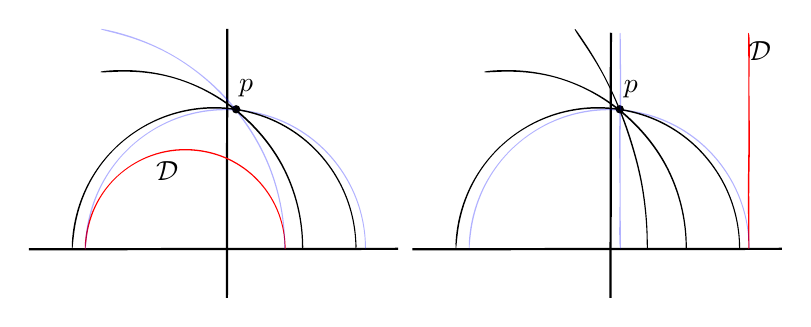
\begin{tikzpicture}[y=0.80pt, x=0.8pt,yscale=-1,scale=0.3, inner sep=0pt, outer sep=0pt]
\begin{scope}[shift={(403.05433,-392.7279)}]% layer1
  % path1866
  \path[draw=black,line join=miter,line cap=butt,line width=0.800pt]
    (-403.0538,724.6608) -- (153.0999,724.0668);

  % path1870
  \path[draw=black,line join=miter,line cap=butt,line width=0.800pt]
    (-104.7851,797.7101) -- (-104.2153,392.7286);

  % path1878
  \path[cm={{0.58173,0.0,0.0,-0.58173,(1587.1216,1835.2022)}},color=black,fill=cff0000,line
    width=0.800pt] (-3275.5852,1929.8550) .. controls (-3273.0523,1957.4390) and
    (-3266.3076,1984.6135) .. (-3255.4343,2010.0642) .. controls
    (-3242.3022,2040.7978) and (-3223.2144,2068.9779) .. (-3199.4833,2092.5040) ..
    controls (-3199.4833,2092.5040) and (-3199.4833,2092.5040) ..
    (-3199.4833,2092.5040) .. controls (-3196.5849,2095.3774) and
    (-3193.6177,2098.1808) .. (-3190.5852,2100.9114) .. controls
    (-3168.8119,2120.5171) and (-3143.8431,2136.5740) .. (-3116.8672,2148.0384) ..
    controls (-3085.0325,2161.5663) and (-3050.4287,2168.6009) ..
    (-3015.8189,2168.5211) .. controls (-3015.8189,2168.5211) and
    (-3015.8189,2168.5211) .. (-3015.8188,2168.5211) .. controls
    (-3014.5342,2168.5211) and (-3013.2496,2168.5051) .. (-3011.9652,2168.4831) ..
    controls (-2978.6525,2167.8984) and (-2945.4166,2161.2569) ..
    (-2914.5853,2148.4764) .. controls (-2885.0650,2136.2376) and
    (-2857.8058,2118.4172) .. (-2834.8876,2096.1108) .. controls
    (-2833.8167,2095.0685) and (-2832.7549,2094.0170) .. (-2831.7023,2092.9564) ..
    controls (-2831.7023,2092.9564) and (-2831.7023,2092.9564) ..
    (-2831.7023,2092.9564) .. controls (-2808.1103,2069.1839) and
    (-2789.1740,2040.8528) .. (-2776.3357,2010.0084) .. controls
    (-2764.6873,1982.0194) and (-2758.1257,1951.9978) .. (-2756.8673,1921.8152) ..
    controls (-2756.3541,1917.3422) and (-2756.3886,1914.0326) ..
    (-2756.6428,1911.8835) .. controls (-2756.8970,1909.7345) and
    (-2757.3712,1908.7417) .. (-2757.8323,1908.8474) .. controls
    (-2758.2933,1908.9531) and (-2758.7420,1910.1541) .. (-2759.0288,1912.3943) ..
    controls (-2759.3156,1914.6345) and (-2759.4411,1917.9117) ..
    (-2759.3283,1922.2139) .. controls (-2760.7024,1951.9336) and
    (-2767.2693,1981.4640) .. (-2778.7998,2008.9662) .. controls
    (-2791.5811,2039.4553) and (-2810.3934,2067.4377) .. (-2833.7762,2090.8825) ..
    controls (-2833.7762,2090.8825) and (-2833.7762,2090.8825) ..
    (-2833.7762,2090.8825) .. controls (-2834.5257,2091.6340) and
    (-2835.2800,2092.3809) .. (-2836.0389,2093.1231) .. controls
    (-2858.9427,2115.5228) and (-2886.2652,2133.3648) .. (-2915.8290,2145.5361) ..
    controls (-2945.3655,2157.6979) and (-2977.1181,2164.1657) ..
    (-3008.9742,2165.0464) .. controls (-3011.2478,2165.1094) and
    (-3013.5298,2165.1434) .. (-3015.8188,2165.1468) .. controls
    (-3032.4335,2165.1748) and (-3049.4315,2163.6142) .. (-3066.2781,2160.3501) ..
    controls (-3083.1247,2157.0860) and (-3099.8145,2152.1178) ..
    (-3115.7905,2145.4929) .. controls (-3129.5679,2139.7805) and
    (-3142.8106,2132.8533) .. (-3155.2346,2124.9376) .. controls
    (-3167.6586,2117.0219) and (-3179.2619,2108.1194) .. (-3189.8265,2098.5206) ..
    controls (-3192.5762,2096.0223) and (-3195.2531,2093.4739) ..
    (-3197.8577,2090.8786) .. controls (-3197.8577,2090.8786) and
    (-3197.8577,2090.8786) .. (-3197.8577,2090.8786) .. controls
    (-3209.9144,2078.8654) and (-3220.4278,2065.8654) .. (-3229.5183,2052.1385) ..
    controls (-3238.6087,2038.4115) and (-3246.2808,2023.9536) ..
    (-3252.5648,2008.8507) .. controls (-3257.2834,1997.5117) and
    (-3261.2087,1985.8062) .. (-3264.3547,1973.7498) .. controls
    (-3267.5007,1961.6933) and (-3269.8684,1949.2848) .. (-3271.4102,1936.5220) ..
    controls (-3271.6958,1934.2846) and (-3272.0403,1931.5842) ..
    (-3272.3805,1928.7519) .. controls (-3272.7206,1925.9195) and
    (-3273.0558,1922.9552) .. (-3273.3642,1920.1958) .. controls
    (-3273.9808,1914.6770) and (-3274.4823,1909.9735) .. (-3275.0562,1908.8398) ..
    controls (-3275.2251,1908.5061) and (-3275.4009,1908.4822) ..
    (-3275.5824,1908.8398) .. controls (-3275.5824,1908.8398) and
    (-3275.5824,1908.8398) .. (-3275.5824,1908.8398) .. controls
    (-3275.7566,1909.1829) and (-3275.9364,1909.8771) .. (-3276.1111,1910.9865) ..
    controls (-3276.3025,1913.7597) and (-3276.3140,1916.9198) ..
    (-3276.2011,1920.1641) .. controls (-3276.0880,1923.4082) and
    (-3275.8503,1926.7360) .. (-3275.5852,1929.8550) -- cycle;

  % path1916-3
  \path[shift={(1200.7271,-935.113)},fill=black,nonzero rule]
    (-1285.2569,1449.0822) .. controls (-1285.2569,1452.5629) and
    (-1288.0786,1455.3846) .. (-1291.5593,1455.3846) .. controls
    (-1295.0401,1455.3846) and (-1297.8618,1452.5629) .. (-1297.8618,1449.0822) ..
    controls (-1297.8618,1445.6014) and (-1295.0401,1442.7797) ..
    (-1291.5593,1442.7797) .. controls (-1288.0786,1442.7797) and
    (-1285.2569,1445.6014) .. (-1285.2569,1449.0822) -- cycle;

  % path1932
  \path[cm={{1.29982,0.0,0.0,-1.29982,(3566.5064,3205.7308)}},color=black,fill=c0000ff,opacity=0.300,line
    width=0.800pt] (-2961.5150,2162.5697) .. controls (-2948.1268,2159.5387) and
    (-2934.9597,2155.5354) .. (-2922.1724,2150.5404) .. controls
    (-2909.3852,2145.5453) and (-2896.9782,2139.5575) .. (-2885.1516,2132.5704) ..
    controls (-2883.9420,2131.8558) and (-2882.7385,2131.1308) ..
    (-2881.5413,2130.3955) .. controls (-2869.4887,2122.9932) and
    (-2857.9974,2114.6736) .. (-2847.2395,2105.4792) .. controls
    (-2836.4817,2096.2848) and (-2826.4584,2086.2144) .. (-2817.3838,2075.3463) ..
    controls (-2817.0067,2074.8946) and (-2816.6311,2074.4415) ..
    (-2816.2573,2073.9871) .. controls (-2807.0754,2062.8261) and
    (-2798.7072,2050.9888) .. (-2791.3705,2038.5255) .. controls
    (-2784.0338,2026.0621) and (-2777.7310,2012.9712) .. (-2772.7309,1999.3959) ..
    controls (-2772.6549,1999.1905) and (-2772.5798,1998.9850) ..
    (-2772.5047,1998.7793) .. controls (-2762.6503,1971.8086) and
    (-2757.4203,1943.2002) .. (-2757.0351,1914.5966) .. controls
    (-2756.6747,1910.6180) and (-2757.1438,1908.7490) .. (-2757.5771,1908.8430) ..
    controls (-2758.0105,1908.9370) and (-2758.4131,1910.9721) ..
    (-2758.1858,1914.8033) .. controls (-2758.6701,1943.2007) and
    (-2763.9560,1971.5755) .. (-2773.8008,1998.2999) .. controls
    (-2773.8008,1998.2999) and (-2773.8008,1998.2999) .. (-2773.8008,1998.2999) ..
    controls (-2773.8118,1998.3309) and (-2773.8238,1998.3609) ..
    (-2773.8348,1998.3919) .. controls (-2778.7680,2011.7677) and
    (-2784.9748,2024.6666) .. (-2792.1873,2036.9520) .. controls
    (-2799.3997,2049.2374) and (-2807.6153,2060.9108) .. (-2816.6165,2071.9285) ..
    controls (-2817.2707,2072.7292) and (-2817.9315,2073.5289) ..
    (-2818.5990,2074.3272) .. controls (-2827.4507,2084.9144) and
    (-2837.5006,2095.2540) .. (-2848.3378,2104.6703) .. controls
    (-2859.1749,2114.0865) and (-2870.7920,2122.5715) .. (-2882.4956,2129.7226) ..
    controls (-2883.5611,2130.3736) and (-2884.6277,2131.0127) ..
    (-2885.6955,2131.6405) .. controls (-2897.3336,2138.4826) and
    (-2909.0889,2143.9835) .. (-2921.1648,2148.6372) .. controls
    (-2933.2407,2153.2908) and (-2945.6445,2157.1029) .. (-2958.8250,2160.2778) ..
    controls (-2961.3378,2160.9021) and (-2965.1830,2161.8893) ..
    (-2967.8528,2162.6649) .. controls (-2970.5226,2163.4405) and
    (-2972.0103,2164.0522) .. (-2969.7382,2164.0426) .. controls
    (-2967.2879,2163.8045) and (-2964.2202,2163.1617) .. (-2961.5150,2162.5697) --
    cycle;

  % path1878-2
  \path[cm={{0.81498,0.0,0.0,-0.81498,(2351.3006,2280.3717)}},color=black,fill=c0000ff,opacity=0.300,line
    width=0.800pt] (-3274.9436,1929.8032) .. controls (-3272.5080,1957.3269) and
    (-3265.8220,1984.4645) .. (-3254.9966,2009.8790) .. controls
    (-3241.9225,2040.5697) and (-3222.8788,2068.7120) .. (-3199.2133,2092.2340) ..
    controls (-3199.2133,2092.2340) and (-3199.2133,2092.2341) ..
    (-3199.2133,2092.2341) .. controls (-3196.3229,2095.1069) and
    (-3193.3640,2097.9104) .. (-3190.3400,2100.6418) .. controls
    (-3168.6275,2120.2534) and (-3143.6807,2136.2903) .. (-3116.7349,2147.7256) ..
    controls (-3084.9362,2161.2194) and (-3050.3801,2168.2129) ..
    (-3015.8189,2168.1571) .. controls (-3015.8189,2168.1571) and
    (-3015.8189,2168.1571) .. (-3015.8188,2168.1571) .. controls
    (-3014.5360,2168.1571) and (-3013.2532,2168.1431) .. (-3011.9706,2168.1221) ..
    controls (-2978.7038,2167.5650) and (-2945.5179,2160.8544) ..
    (-2914.7732,2148.0324) .. controls (-2885.3350,2135.7542) and
    (-2858.1816,2117.9258) .. (-2835.2897,2095.6947) .. controls
    (-2834.2200,2094.6559) and (-2833.1594,2093.6079) .. (-2832.1079,2092.5508) ..
    controls (-2832.1079,2092.5508) and (-2832.1079,2092.5508) ..
    (-2832.1079,2092.5508) .. controls (-2808.5412,2068.8578) and
    (-2789.6029,2040.6101) .. (-2776.7337,2009.8402) .. controls
    (-2765.0572,1981.9193) and (-2758.4418,1951.9539) .. (-2757.1094,1921.8032) ..
    controls (-2756.6831,1917.3300) and (-2756.6902,1914.0273) ..
    (-2756.8605,1911.8811) .. controls (-2757.0309,1909.7348) and
    (-2757.3651,1908.7418) .. (-2757.6878,1908.8475) .. controls
    (-2758.0106,1908.9533) and (-2758.3227,1910.1556) .. (-2758.5328,1912.4012) ..
    controls (-2758.7430,1914.6469) and (-2758.8518,1917.9343) ..
    (-2758.8402,1922.2394) .. controls (-2760.2690,1952.0128) and
    (-2766.8850,1981.5788) .. (-2778.4586,2009.1106) .. controls
    (-2791.2879,2039.6320) and (-2810.1396,2067.6357) .. (-2833.5596,2091.0991) ..
    controls (-2833.5596,2091.0991) and (-2833.5596,2091.0991) ..
    (-2833.5596,2091.0991) .. controls (-2834.3104,2091.8513) and
    (-2835.0658,2092.5987) .. (-2835.8259,2093.3415) .. controls
    (-2858.7655,2115.7590) and (-2886.0603,2133.6947) .. (-2915.6437,2145.9742) ..
    controls (-2945.2005,2158.2439) and (-2977.0197,2164.8233) ..
    (-3008.9568,2165.6973) .. controls (-3011.2362,2165.7593) and
    (-3013.5240,2165.7923) .. (-3015.8188,2165.7953) .. controls
    (-3032.4756,2165.8143) and (-3049.5140,2164.2288) .. (-3066.3936,2160.9292) ..
    controls (-3083.2731,2157.6295) and (-3099.9883,2152.6158) ..
    (-3115.9812,2145.9441) .. controls (-3129.7729,2140.1911) and
    (-3143.0226,2133.2229) .. (-3155.4494,2125.2700) .. controls
    (-3167.8762,2117.3171) and (-3179.4780,2108.3813) .. (-3190.0419,2098.7557) ..
    controls (-3192.7914,2096.2503) and (-3195.4690,2093.6963) ..
    (-3198.0754,2091.0965) .. controls (-3198.0754,2091.0965) and
    (-3198.0754,2091.0965) .. (-3198.0754,2091.0965) .. controls
    (-3210.1400,2079.0623) and (-3220.6827,2066.0640) .. (-3229.8131,2052.3368) ..
    controls (-3238.9435,2038.6095) and (-3246.6658,2024.1490) ..
    (-3252.9879,2009.0298) .. controls (-3257.7350,1997.6784) and
    (-3261.6813,1985.9537) .. (-3264.8295,1973.8733) .. controls
    (-3267.9776,1961.7929) and (-3270.3284,1949.3554) .. (-3271.8235,1936.5668) ..
    controls (-3272.0964,1934.3244) and (-3272.4159,1931.6173) ..
    (-3272.7203,1928.7784) .. controls (-3273.0246,1925.9395) and
    (-3273.3132,1922.9689) .. (-3273.5657,1920.2049) .. controls
    (-3274.0707,1914.6768) and (-3274.4236,1909.9727) .. (-3274.8254,1908.8400) ..
    controls (-3274.9436,1908.5066) and (-3275.0667,1908.4830) ..
    (-3275.1938,1908.8400) .. controls (-3275.1938,1908.8400) and
    (-3275.1938,1908.8400) .. (-3275.1938,1908.8400) .. controls
    (-3275.3157,1909.1825) and (-3275.4416,1909.8755) .. (-3275.5612,1910.9822) ..
    controls (-3275.6884,1913.7490) and (-3275.6746,1916.9003) ..
    (-3275.5512,1920.1361) .. controls (-3275.4325,1923.3716) and
    (-3275.2040,1926.6916) .. (-3274.9436,1929.8032) -- cycle;

  % path2054
  \path[cm={{0.82575,0.0,0.0,-0.82575,(2366.591,2300.93)}},color=black,fill=black,line
    width=0.800pt] (-3275.1575,1929.8205) .. controls (-3272.6894,1957.3643) and
    (-3265.9839,1984.5141) .. (-3255.1425,2009.9408) .. controls
    (-3242.0491,2040.6458) and (-3222.9907,2068.8007) .. (-3199.3033,2092.3240) ..
    controls (-3199.3033,2092.3240) and (-3199.3033,2092.3240) ..
    (-3199.3033,2092.3241) .. controls (-3196.4103,2095.1970) and
    (-3193.4485,2098.0006) .. (-3190.4217,2100.7317) .. controls
    (-3168.6890,2120.3413) and (-3143.7349,2136.3849) .. (-3116.7790,2147.8299) ..
    controls (-3084.9683,2161.3350) and (-3050.3963,2168.3422) ..
    (-3015.8189,2168.2784) .. controls (-3015.8189,2168.2784) and
    (-3015.8189,2168.2784) .. (-3015.8188,2168.2784) .. controls
    (-3014.5354,2168.2784) and (-3013.2520,2168.2644) .. (-3011.9688,2168.2424) ..
    controls (-2978.6867,2167.6762) and (-2945.4841,2160.9886) ..
    (-2914.7105,2148.1805) .. controls (-2885.2450,2135.9154) and
    (-2858.0563,2118.0897) .. (-2835.1556,2095.8335) .. controls
    (-2834.0856,2094.7935) and (-2833.0245,2093.7443) .. (-2831.9727,2092.6861) ..
    controls (-2831.9727,2092.6861) and (-2831.9727,2092.6860) ..
    (-2831.9727,2092.6860) .. controls (-2808.3976,2068.9665) and
    (-2789.4599,2040.6911) .. (-2776.6010,2009.8963) .. controls
    (-2764.9339,1981.9527) and (-2758.3364,1951.9686) .. (-2757.0287,1921.8072) ..
    controls (-2756.5734,1917.3341) and (-2756.5896,1914.0291) ..
    (-2756.7880,1911.8819) .. controls (-2756.9863,1909.7347) and
    (-2757.3672,1908.7418) .. (-2757.7360,1908.8475) .. controls
    (-2758.1048,1908.9533) and (-2758.4624,1910.1551) .. (-2758.6982,1912.3990) ..
    controls (-2758.9339,1914.6428) and (-2759.0483,1917.9268) ..
    (-2759.0029,1922.2309) .. controls (-2760.4135,1951.9864) and
    (-2767.0131,1981.5406) .. (-2778.5723,2009.0625) .. controls
    (-2791.3857,2039.5731) and (-2810.2242,2067.5697) .. (-2833.6318,2091.0269) ..
    controls (-2833.6318,2091.0269) and (-2833.6318,2091.0269) ..
    (-2833.6318,2091.0269) .. controls (-2834.3822,2091.7789) and
    (-2835.1372,2092.5262) .. (-2835.8969,2093.2687) .. controls
    (-2858.8246,2115.6803) and (-2886.1286,2133.5847) .. (-2915.7055,2145.8282) ..
    controls (-2945.2555,2158.0619) and (-2977.0525,2164.6041) ..
    (-3008.9626,2165.4804) .. controls (-3011.2401,2165.5434) and
    (-3013.5259,2165.5764) .. (-3015.8188,2165.5794) .. controls
    (-3032.4616,2165.6014) and (-3049.4865,2164.0242) .. (-3066.3551,2160.7364) ..
    controls (-3083.2236,2157.4486) and (-3099.9303,2152.4501) ..
    (-3115.9176,2145.7939) .. controls (-3129.7045,2140.0545) and
    (-3142.9519,2133.0999) .. (-3155.3778,2125.1595) .. controls
    (-3167.8037,2117.2190) and (-3179.4060,2108.2943) .. (-3189.9701,2098.6776) ..
    controls (-3192.7197,2096.1746) and (-3195.3971,2093.6224) ..
    (-3198.0028,2091.0242) .. controls (-3198.0028,2091.0242) and
    (-3198.0028,2091.0242) .. (-3198.0028,2091.0242) .. controls
    (-3210.0648,2078.9970) and (-3220.5978,2065.9980) .. (-3229.7148,2052.2709) ..
    controls (-3238.8319,2038.5438) and (-3246.5375,2024.0841) ..
    (-3252.8469,2008.9704) .. controls (-3257.5845,1997.6231) and
    (-3261.5238,1985.9048) .. (-3264.6712,1973.8324) .. controls
    (-3267.8187,1961.7600) and (-3270.1751,1949.3321) .. (-3271.6857,1936.5521) ..
    controls (-3271.9629,1934.3114) and (-3272.2907,1931.6065) ..
    (-3272.6070,1928.7698) .. controls (-3272.9233,1925.9331) and
    (-3273.2274,1922.9646) .. (-3273.4985,1920.2021) .. controls
    (-3274.0407,1914.6772) and (-3274.4432,1909.9732) .. (-3274.9023,1908.8402) ..
    controls (-3275.0375,1908.5067) and (-3275.1781,1908.4830) ..
    (-3275.3233,1908.8402) .. controls (-3275.3233,1908.8402) and
    (-3275.3233,1908.8402) .. (-3275.3233,1908.8402) .. controls
    (-3275.4627,1909.1829) and (-3275.6065,1909.8763) .. (-3275.7445,1910.9839) ..
    controls (-3275.8931,1913.7528) and (-3275.8877,1916.9070) ..
    (-3275.7695,1920.1457) .. controls (-3275.6510,1923.3838) and
    (-3275.4194,1926.7064) .. (-3275.1575,1929.8205) -- cycle;

  % path2058
  \path[cm={{1.03907,0.0,0.0,-1.03907,(2874.6344,2708.064)}},color=black,fill=black,line
    width=0.800pt] (-3039.5652,2167.7226) .. controls (-3031.6640,2168.3333) and
    (-3023.7399,2168.6126) .. (-3015.8188,2168.5486) .. controls
    (-2988.4128,2168.3274) and (-2961.0045,2163.9925) .. (-2935.0081,2155.3061) ..
    controls (-2928.2137,2153.0358) and (-2921.5071,2150.5046) ..
    (-2914.9112,2147.7058) .. controls (-2888.9769,2136.7008) and
    (-2864.7315,2121.5845) .. (-2843.7054,2102.7949) .. controls
    (-2839.8644,2099.3625) and (-2836.1126,2095.8310) .. (-2832.4591,2092.1993) ..
    controls (-2821.7427,2081.5469) and (-2811.8691,2070.0295) ..
    (-2803.0760,2057.7184) .. controls (-2794.2830,2045.4073) and
    (-2786.5730,2032.3006) .. (-2780.2370,2018.5574) .. controls
    (-2778.9258,2015.7131) and (-2777.6671,2012.8450) .. (-2776.4621,2009.9547) ..
    controls (-2764.0382,1980.1506) and (-2757.4095,1948.0200) ..
    (-2756.8808,1915.8816) .. controls (-2756.3438,1911.0189) and
    (-2757.0424,1908.7289) .. (-2757.6878,1908.8437) .. controls
    (-2758.3333,1908.9586) and (-2758.9329,1911.4384) .. (-2758.5943,1916.1186) ..
    controls (-2759.2568,1947.9476) and (-2765.9482,1979.7278) ..
    (-2778.3322,2009.1638) .. controls (-2779.4491,2011.8188) and
    (-2780.6118,2014.4546) .. (-2781.8191,2017.0700) .. controls
    (-2788.1592,2030.8039) and (-2795.8856,2043.8914) .. (-2804.6937,2056.1744) ..
    controls (-2813.5018,2068.4573) and (-2823.3890,2079.9374) ..
    (-2834.1085,2090.5499) .. controls (-2837.3440,2093.7532) and
    (-2840.6560,2096.8780) .. (-2844.0377,2099.9253) .. controls
    (-2854.2657,2109.1417) and (-2865.5812,2117.9245) .. (-2877.6477,2125.7688) ..
    controls (-2889.7143,2133.6131) and (-2902.5269,2140.5133) ..
    (-2915.5651,2146.1597) .. controls (-2922.3639,2149.1043) and
    (-2929.2207,2151.7085) .. (-2936.0447,2153.9676) .. controls
    (-2949.3550,2158.3741) and (-2962.5647,2161.3507) .. (-2975.7898,2163.2910) ..
    controls (-2989.0149,2165.2313) and (-3002.2625,2166.1385) ..
    (-3015.8188,2166.1644) .. controls (-3022.3119,2166.1764) and
    (-3028.8779,2165.9830) .. (-3035.5554,2165.5799) .. controls
    (-3038.7126,2165.4169) and (-3043.5576,2165.2125) .. (-3046.9626,2165.1985) ..
    controls (-3048.6651,2165.1885) and (-3050.0081,2165.2425) ..
    (-3050.5980,2165.4191) .. controls (-3051.1879,2165.5954) and
    (-3051.0254,2165.9011) .. (-3049.7056,2166.3709) .. controls
    (-3046.7665,2167.0602) and (-3042.9442,2167.4315) .. (-3039.5652,2167.7226) --
    cycle;

  % path1880
  \path[draw=black,line join=miter,line cap=butt,line width=0.800pt]
    (174.5463,724.6608) -- (730.7000,724.0668);

  % path1882
  \path[draw=black,line join=miter,line cap=butt,line width=0.800pt]
    (472.8150,797.7101) -- (473.3848,398.7051);

  % path2043
  \path[fill=cff0000] (679.8680,407.1633) .. controls (680.3286,433.0809) and
    (680.1938,459.0359) .. (680.3833,485.0150) .. controls (680.5728,510.9939) and
    (680.1765,536.9941) .. (680.2544,562.9991) .. controls (680.3323,589.0041) and
    (679.4845,615.0114) .. (679.6102,641.0072) .. controls (679.7359,667.0026) and
    (679.9253,692.9848) .. (680.2583,718.9356) .. controls (679.4364,726.1109) and
    (682.8944,725.6481) .. (681.9649,718.7285) .. controls (681.7506,693.0150) and
    (681.6837,667.2694) .. (681.6713,641.5126) .. controls (681.6589,615.7558) and
    (682.6106,589.9897) .. (682.6139,564.2320) .. controls (682.6169,538.4742) and
    (682.1451,510.3128) .. (681.9779,484.5964) .. controls (681.8107,458.8800) and
    (682.8588,435.6119) .. (682.3350,409.9792) .. controls (682.1844,405.2990) and
    (681.2815,395.6398) .. (680.0999,399.6595) .. controls (679.7960,401.8637) and
    (679.8536,404.6761) .. (679.8680,407.1633) -- cycle;

  % path1893
  \path[shift={(1778.3272,-935.113)},fill=black,nonzero rule]
    (-1285.2569,1449.0822) .. controls (-1285.2569,1452.5629) and
    (-1288.0786,1455.3846) .. (-1291.5593,1455.3846) .. controls
    (-1295.0401,1455.3846) and (-1297.8618,1452.5629) .. (-1297.8618,1449.0822) ..
    controls (-1297.8618,1445.6014) and (-1295.0401,1442.7797) ..
    (-1291.5593,1442.7797) .. controls (-1288.0786,1442.7797) and
    (-1285.2569,1445.6014) .. (-1285.2569,1449.0822) -- cycle;

  % path1913
  \path[cm={{0.81498,0.0,0.0,-0.81498,(2928.9007,2280.3717)}},color=black,fill=c0000ff,opacity=0.300,line
    width=0.800pt] (-3274.9436,1929.8032) .. controls (-3272.5080,1957.3269) and
    (-3265.8220,1984.4645) .. (-3254.9966,2009.8790) .. controls
    (-3241.9225,2040.5697) and (-3222.8788,2068.7120) .. (-3199.2133,2092.2340) ..
    controls (-3199.2133,2092.2340) and (-3199.2133,2092.2341) ..
    (-3199.2133,2092.2341) .. controls (-3196.3229,2095.1069) and
    (-3193.3640,2097.9104) .. (-3190.3400,2100.6418) .. controls
    (-3168.6275,2120.2534) and (-3143.6807,2136.2903) .. (-3116.7349,2147.7256) ..
    controls (-3084.9362,2161.2194) and (-3050.3801,2168.2129) ..
    (-3015.8189,2168.1571) .. controls (-3015.8189,2168.1571) and
    (-3015.8189,2168.1571) .. (-3015.8188,2168.1571) .. controls
    (-3014.5360,2168.1571) and (-3013.2532,2168.1431) .. (-3011.9706,2168.1221) ..
    controls (-2978.7038,2167.5650) and (-2945.5179,2160.8544) ..
    (-2914.7732,2148.0324) .. controls (-2885.3350,2135.7542) and
    (-2858.1816,2117.9258) .. (-2835.2897,2095.6947) .. controls
    (-2834.2200,2094.6559) and (-2833.1594,2093.6079) .. (-2832.1079,2092.5508) ..
    controls (-2832.1079,2092.5508) and (-2832.1079,2092.5508) ..
    (-2832.1079,2092.5508) .. controls (-2808.5412,2068.8578) and
    (-2789.6029,2040.6101) .. (-2776.7337,2009.8402) .. controls
    (-2765.0572,1981.9193) and (-2758.4418,1951.9539) .. (-2757.1094,1921.8032) ..
    controls (-2756.6831,1917.3300) and (-2756.6902,1914.0273) ..
    (-2756.8605,1911.8811) .. controls (-2757.0309,1909.7348) and
    (-2757.3651,1908.7418) .. (-2757.6878,1908.8475) .. controls
    (-2758.0106,1908.9533) and (-2758.3227,1910.1556) .. (-2758.5328,1912.4012) ..
    controls (-2758.7430,1914.6469) and (-2758.8518,1917.9343) ..
    (-2758.8402,1922.2394) .. controls (-2760.2690,1952.0128) and
    (-2766.8850,1981.5788) .. (-2778.4586,2009.1106) .. controls
    (-2791.2879,2039.6320) and (-2810.1396,2067.6357) .. (-2833.5596,2091.0991) ..
    controls (-2833.5596,2091.0991) and (-2833.5596,2091.0991) ..
    (-2833.5596,2091.0991) .. controls (-2834.3104,2091.8513) and
    (-2835.0658,2092.5987) .. (-2835.8259,2093.3415) .. controls
    (-2858.7655,2115.7590) and (-2886.0603,2133.6947) .. (-2915.6437,2145.9742) ..
    controls (-2945.2005,2158.2439) and (-2977.0197,2164.8233) ..
    (-3008.9568,2165.6973) .. controls (-3011.2362,2165.7593) and
    (-3013.5240,2165.7923) .. (-3015.8188,2165.7953) .. controls
    (-3032.4756,2165.8143) and (-3049.5140,2164.2288) .. (-3066.3936,2160.9292) ..
    controls (-3083.2731,2157.6295) and (-3099.9883,2152.6158) ..
    (-3115.9812,2145.9441) .. controls (-3129.7729,2140.1911) and
    (-3143.0226,2133.2229) .. (-3155.4494,2125.2700) .. controls
    (-3167.8762,2117.3171) and (-3179.4780,2108.3813) .. (-3190.0419,2098.7557) ..
    controls (-3192.7914,2096.2503) and (-3195.4690,2093.6963) ..
    (-3198.0754,2091.0965) .. controls (-3198.0754,2091.0965) and
    (-3198.0754,2091.0965) .. (-3198.0754,2091.0965) .. controls
    (-3210.1400,2079.0623) and (-3220.6827,2066.0640) .. (-3229.8131,2052.3368) ..
    controls (-3238.9435,2038.6095) and (-3246.6658,2024.1490) ..
    (-3252.9879,2009.0298) .. controls (-3257.7350,1997.6784) and
    (-3261.6813,1985.9537) .. (-3264.8295,1973.8733) .. controls
    (-3267.9776,1961.7929) and (-3270.3284,1949.3554) .. (-3271.8235,1936.5668) ..
    controls (-3272.0964,1934.3244) and (-3272.4159,1931.6173) ..
    (-3272.7203,1928.7784) .. controls (-3273.0246,1925.9395) and
    (-3273.3132,1922.9689) .. (-3273.5657,1920.2049) .. controls
    (-3274.0707,1914.6768) and (-3274.4236,1909.9727) .. (-3274.8254,1908.8400) ..
    controls (-3274.9436,1908.5066) and (-3275.0667,1908.4830) ..
    (-3275.1938,1908.8400) .. controls (-3275.1938,1908.8400) and
    (-3275.1938,1908.8400) .. (-3275.1938,1908.8400) .. controls
    (-3275.3157,1909.1825) and (-3275.4416,1909.8755) .. (-3275.5612,1910.9822) ..
    controls (-3275.6884,1913.7490) and (-3275.6746,1916.9003) ..
    (-3275.5512,1920.1361) .. controls (-3275.4325,1923.3716) and
    (-3275.2040,1926.6916) .. (-3274.9436,1929.8032) -- cycle;

  % path1917
  \path[cm={{0.82575,0.0,0.0,-0.82575,(2944.1911,2300.93)}},color=black,fill=black,line
    width=0.800pt] (-3275.1575,1929.8205) .. controls (-3272.6894,1957.3643) and
    (-3265.9839,1984.5141) .. (-3255.1425,2009.9408) .. controls
    (-3242.0491,2040.6458) and (-3222.9907,2068.8007) .. (-3199.3033,2092.3240) ..
    controls (-3199.3033,2092.3240) and (-3199.3033,2092.3240) ..
    (-3199.3033,2092.3241) .. controls (-3196.4103,2095.1970) and
    (-3193.4485,2098.0006) .. (-3190.4217,2100.7317) .. controls
    (-3168.6890,2120.3413) and (-3143.7349,2136.3849) .. (-3116.7790,2147.8299) ..
    controls (-3084.9683,2161.3350) and (-3050.3963,2168.3422) ..
    (-3015.8189,2168.2784) .. controls (-3015.8189,2168.2784) and
    (-3015.8189,2168.2784) .. (-3015.8188,2168.2784) .. controls
    (-3014.5354,2168.2784) and (-3013.2520,2168.2644) .. (-3011.9688,2168.2424) ..
    controls (-2978.6867,2167.6762) and (-2945.4841,2160.9886) ..
    (-2914.7105,2148.1805) .. controls (-2885.2450,2135.9154) and
    (-2858.0563,2118.0897) .. (-2835.1556,2095.8335) .. controls
    (-2834.0856,2094.7935) and (-2833.0245,2093.7443) .. (-2831.9727,2092.6861) ..
    controls (-2831.9727,2092.6861) and (-2831.9727,2092.6860) ..
    (-2831.9727,2092.6860) .. controls (-2808.3976,2068.9665) and
    (-2789.4599,2040.6911) .. (-2776.6010,2009.8963) .. controls
    (-2764.9339,1981.9527) and (-2758.3364,1951.9686) .. (-2757.0287,1921.8072) ..
    controls (-2756.5734,1917.3341) and (-2756.5896,1914.0291) ..
    (-2756.7880,1911.8819) .. controls (-2756.9863,1909.7347) and
    (-2757.3672,1908.7418) .. (-2757.7360,1908.8475) .. controls
    (-2758.1048,1908.9533) and (-2758.4624,1910.1551) .. (-2758.6982,1912.3990) ..
    controls (-2758.9339,1914.6428) and (-2759.0483,1917.9268) ..
    (-2759.0029,1922.2309) .. controls (-2760.4135,1951.9864) and
    (-2767.0131,1981.5406) .. (-2778.5723,2009.0625) .. controls
    (-2791.3857,2039.5731) and (-2810.2242,2067.5697) .. (-2833.6318,2091.0269) ..
    controls (-2833.6318,2091.0269) and (-2833.6318,2091.0269) ..
    (-2833.6318,2091.0269) .. controls (-2834.3822,2091.7789) and
    (-2835.1372,2092.5262) .. (-2835.8969,2093.2687) .. controls
    (-2858.8246,2115.6803) and (-2886.1286,2133.5847) .. (-2915.7055,2145.8282) ..
    controls (-2945.2555,2158.0619) and (-2977.0525,2164.6041) ..
    (-3008.9626,2165.4804) .. controls (-3011.2401,2165.5434) and
    (-3013.5259,2165.5764) .. (-3015.8188,2165.5794) .. controls
    (-3032.4616,2165.6014) and (-3049.4865,2164.0242) .. (-3066.3551,2160.7364) ..
    controls (-3083.2236,2157.4486) and (-3099.9303,2152.4501) ..
    (-3115.9176,2145.7939) .. controls (-3129.7045,2140.0545) and
    (-3142.9519,2133.0999) .. (-3155.3778,2125.1595) .. controls
    (-3167.8037,2117.2190) and (-3179.4060,2108.2943) .. (-3189.9701,2098.6776) ..
    controls (-3192.7197,2096.1746) and (-3195.3971,2093.6224) ..
    (-3198.0028,2091.0242) .. controls (-3198.0028,2091.0242) and
    (-3198.0028,2091.0242) .. (-3198.0028,2091.0242) .. controls
    (-3210.0648,2078.9970) and (-3220.5978,2065.9980) .. (-3229.7148,2052.2709) ..
    controls (-3238.8319,2038.5438) and (-3246.5375,2024.0841) ..
    (-3252.8469,2008.9704) .. controls (-3257.5845,1997.6231) and
    (-3261.5238,1985.9048) .. (-3264.6712,1973.8324) .. controls
    (-3267.8187,1961.7600) and (-3270.1751,1949.3321) .. (-3271.6857,1936.5521) ..
    controls (-3271.9629,1934.3114) and (-3272.2907,1931.6065) ..
    (-3272.6070,1928.7698) .. controls (-3272.9233,1925.9331) and
    (-3273.2274,1922.9646) .. (-3273.4985,1920.2021) .. controls
    (-3274.0407,1914.6772) and (-3274.4432,1909.9732) .. (-3274.9023,1908.8402) ..
    controls (-3275.0375,1908.5067) and (-3275.1781,1908.4830) ..
    (-3275.3233,1908.8402) .. controls (-3275.3233,1908.8402) and
    (-3275.3233,1908.8402) .. (-3275.3233,1908.8402) .. controls
    (-3275.4627,1909.1829) and (-3275.6065,1909.8763) .. (-3275.7445,1910.9839) ..
    controls (-3275.8931,1913.7528) and (-3275.8877,1916.9070) ..
    (-3275.7695,1920.1457) .. controls (-3275.6510,1923.3838) and
    (-3275.4194,1926.7064) .. (-3275.1575,1929.8205) -- cycle;

  % path1921
  \path[cm={{1.03907,0.0,0.0,-1.03907,(3452.2345,2708.064)}},color=black,fill=black,line
    width=0.800pt] (-3039.5652,2167.7226) .. controls (-3031.6640,2168.3333) and
    (-3023.7399,2168.6126) .. (-3015.8188,2168.5486) .. controls
    (-2988.4128,2168.3274) and (-2961.0045,2163.9925) .. (-2935.0081,2155.3061) ..
    controls (-2928.2137,2153.0358) and (-2921.5071,2150.5046) ..
    (-2914.9112,2147.7058) .. controls (-2888.9769,2136.7008) and
    (-2864.7315,2121.5845) .. (-2843.7054,2102.7949) .. controls
    (-2839.8644,2099.3625) and (-2836.1126,2095.8310) .. (-2832.4591,2092.1993) ..
    controls (-2821.7427,2081.5469) and (-2811.8691,2070.0295) ..
    (-2803.0760,2057.7184) .. controls (-2794.2830,2045.4073) and
    (-2786.5730,2032.3006) .. (-2780.2370,2018.5574) .. controls
    (-2778.9258,2015.7131) and (-2777.6671,2012.8450) .. (-2776.4621,2009.9547) ..
    controls (-2764.0382,1980.1506) and (-2757.4095,1948.0200) ..
    (-2756.8808,1915.8816) .. controls (-2756.3438,1911.0189) and
    (-2757.0424,1908.7289) .. (-2757.6878,1908.8437) .. controls
    (-2758.3333,1908.9586) and (-2758.9329,1911.4384) .. (-2758.5943,1916.1186) ..
    controls (-2759.2568,1947.9476) and (-2765.9482,1979.7278) ..
    (-2778.3322,2009.1638) .. controls (-2779.4491,2011.8188) and
    (-2780.6118,2014.4546) .. (-2781.8191,2017.0700) .. controls
    (-2788.1592,2030.8039) and (-2795.8856,2043.8914) .. (-2804.6937,2056.1744) ..
    controls (-2813.5018,2068.4573) and (-2823.3890,2079.9374) ..
    (-2834.1085,2090.5499) .. controls (-2837.3440,2093.7532) and
    (-2840.6560,2096.8780) .. (-2844.0377,2099.9253) .. controls
    (-2854.2657,2109.1417) and (-2865.5812,2117.9245) .. (-2877.6477,2125.7688) ..
    controls (-2889.7143,2133.6131) and (-2902.5269,2140.5133) ..
    (-2915.5651,2146.1597) .. controls (-2922.3639,2149.1043) and
    (-2929.2207,2151.7085) .. (-2936.0447,2153.9676) .. controls
    (-2949.3550,2158.3741) and (-2962.5647,2161.3507) .. (-2975.7898,2163.2910) ..
    controls (-2989.0149,2165.2313) and (-3002.2625,2166.1385) ..
    (-3015.8188,2166.1644) .. controls (-3022.3119,2166.1764) and
    (-3028.8779,2165.9830) .. (-3035.5554,2165.5799) .. controls
    (-3038.7126,2165.4169) and (-3043.5576,2165.2125) .. (-3046.9626,2165.1985) ..
    controls (-3048.6651,2165.1885) and (-3050.0081,2165.2425) ..
    (-3050.5980,2165.4191) .. controls (-3051.1879,2165.5954) and
    (-3051.0254,2165.9011) .. (-3049.7056,2166.3709) .. controls
    (-3046.7665,2167.0602) and (-3042.9442,2167.4315) .. (-3039.5652,2167.7226) --
    cycle;

  \begin{scope}% g1192
    % text1898
    \path[fill=black] (-211.42528,621.1048) node[above right] (text1898)
      {$\mathcal{D}$};

    % text2048
    \path[fill=black] (-86.336166,495.55255) node[above right] (text2048) {$p$};

    % text1888
    \path[fill=black] (681.02979,440.63895) node[above right] (text1888)
      {$\mathcal{D}$};

    % text2052
    \path[fill=black] (493.04617,496.52493) node[above right] (text2052) {$p$};

  \end{scope}
  % path888
  \path[fill=c0000ff,opacity=0.300] (488.5432,715.6605) .. controls
    (488.0826,689.7428) and (488.2175,663.7879) .. (488.0279,637.8087) .. controls
    (487.8384,611.8298) and (488.2348,585.8297) .. (488.1569,559.8247) .. controls
    (488.0790,533.8197) and (488.9268,507.8123) .. (488.8011,481.8165) .. controls
    (488.6754,455.8211) and (488.4859,429.8389) .. (488.1529,403.8882) .. controls
    (488.9748,396.7128) and (485.5168,397.1756) .. (486.4463,404.0953) .. controls
    (486.6607,429.8087) and (486.7275,455.5543) .. (486.7400,481.3111) .. controls
    (486.7524,507.0679) and (485.8006,532.8340) .. (485.7973,558.5918) .. controls
    (485.7943,584.3496) and (486.2661,612.5110) .. (486.4333,638.2274) .. controls
    (486.6005,663.9438) and (485.5524,687.2119) .. (486.0762,712.8445) .. controls
    (486.2269,717.5247) and (487.1297,727.1839) .. (488.3113,723.1643) .. controls
    (488.6152,720.9601) and (488.5576,718.1477) .. (488.5432,715.6605) -- cycle;

  % path892
  \path[cm={{2.14135,0.0,0.0,-2.14135,(6432.8793,4812.1405)}},color=black,fill=black,line
    width=0.800pt] (-2805.7366,2060.5092) .. controls (-2798.1636,2049.6373) and
    (-2791.2317,2038.3045) .. (-2785.3185,2026.4335) .. controls
    (-2779.4053,2014.5626) and (-2774.1639,2002.3274) .. (-2770.0638,1989.6987) ..
    controls (-2765.9636,1977.0701) and (-2762.4318,1964.2176) ..
    (-2760.3099,1951.1068) .. controls (-2758.1880,1937.9962) and
    (-2757.1000,1924.7304) .. (-2757.1224,1911.4852) .. controls
    (-2756.9296,1909.6557) and (-2757.2184,1908.7979) .. (-2757.4953,1908.8412) ..
    controls (-2757.7719,1908.8842) and (-2758.0371,1909.8221) ..
    (-2757.8547,1911.5844) .. controls (-2757.8867,1924.6699) and
    (-2759.0093,1937.7684) .. (-2761.1391,1950.7088) .. controls
    (-2763.2688,1963.6492) and (-2766.7819,1976.3290) .. (-2770.8304,1988.7885) ..
    controls (-2772.8547,1995.0183) and (-2775.1661,2001.4779) ..
    (-2777.7267,2007.8386) .. controls (-2780.2874,2014.1993) and
    (-2783.0970,2020.4599) .. (-2786.0246,2026.3157) .. controls
    (-2788.9523,2032.1714) and (-2792.0687,2037.5805) .. (-2795.3496,2042.8731) ..
    controls (-2798.6305,2048.1658) and (-2802.0756,2053.3433) ..
    (-2805.7619,2058.7265) .. controls (-2806.4253,2059.7162) and
    (-2807.4027,2061.2612) .. (-2808.0220,2062.3858) .. controls
    (-2808.6414,2063.5104) and (-2808.8948,2064.2213) .. (-2808.0790,2063.5474) ..
    controls (-2807.3032,2062.7205) and (-2806.4737,2061.5451) ..
    (-2805.7366,2060.5092) -- cycle;

\end{scope}

\end{tikzpicture}


\end{center}
\pause \footnotesize{Proste zaznaczone na niebiesko, które spotykają się z prostą $D$ w nieskończoności nazywamy \textbf{ultra-równoległymi}.}\hfill $\square$

\end{frame}
%%%%%%next-slide%%%%%

\mode<all>{\lowsection{Aksjomat Pascha}}
\begin{frame}[<+->]
\begin{lemat}
\label{9.2.3}
Jeśli $A=(x_{1},y_{1})$, $B=(x_{2},y_{2})$ są dwoma różnymi punktami półpłaszczyzny Poincar\'{e}go, to dla dowolnej prostej hiperbolicznej $\mathcal{D} \subset \mathcal{H}$ zachodzi równoważność:
\[(\mathcal{D}\cap [AB]\neq \varnothing)\iff \le(f_\mathcal{D}(x_{1},y_{1})\cdot 
f_\mathcal{D}(x_{2},y_{2})\leqslant 0\ri).\]
\end{lemat}

\begin{twierdzenie}[Aksjomat Pascha]
Jeśli $A=(x_{1},y_{1})$, $B=(x_{2},y_{2})$, $C=(x_{3},y_{3})$ są dowolnymi punktami półpłaszczyzny Poincar\'{e}go nieleżącymi na jednej prostej hiperbolicznej oraz pewna prosta hiperboliczna $\mathcal{D}$ przecina jeden z odcinków hiperbolicznych $[AB]$, $[BC]$ lub $[CA]$, to przecina ona jeszcze co najmniej jeden z nich.
\end{twierdzenie}

\end{frame}
%%%%%%next-slide%%%%%
\begin{frame}
\textcolor{ared}{\textbf{Dowód:}}\\
Przypuśćmy, że $\mathcal{D}\cap [AB]\neq \varnothing$ oraz $\mathcal{D}\cap [BC]=
\varnothing$ i $\mathcal{D}\cap [CA]=\varnothing$. \pause Wówczas na mocy poprzedniego lematu (\ref{9.2.3}) mamy
\begin{align*}
f_\mathcal{D}(x_{1},y_{1})\cdot f_\mathcal{D}(x_{2},y_{2})&\leqslant 0,\\
f_\mathcal{D}(x_{2},y_{2})\cdot f_\mathcal{D}(x_{3},y_{3})&>0,\\
f_\mathcal{D}(x_{3},y_{3})\cdot f_\mathcal{D}(x_{1},y_{1})&>0.
\end{align*}
\pause Mnożąc stronami dwie ostatnie nierówności dostajemy w wyniku nierówność 
\[f_\mathcal{D}(x_{1},y_{1})\cdot f_\mathcal{D}(x_{2},y_{2})\cdot {(f_\mathcal{D}(x_{3},y_{3}))}^{2}>0.\]
\pause Dzieląc przez ${(f_\mathcal{D}(x_{3},y_{3}))}^{2}$ otrzymujemy 
\[f_\mathcal{D}(x_{1},y_{1})\cdot f_\mathcal{D}(x_{2},y_{2})>0,\] co jest sprzeczne z pierwszą z nierówności.
\hfill $\square$
\end{frame}


\mode<all>{\midsection{Symetrie hiperboliczne}}
\begin{frame}


Z każdą prostą hiperboliczną można stowarzyszyć przekształcenie wzorowane na symetrii osiowej z płaszczyzny euklidesowej. %Będą to przekształcenia wyznaczone przez symetrie osiowe i inwersje względem okręgu.

\pause \begin{definicja} %9.2.10
\label{9.2.10}
\textbf{Symetrią hiperboliczną} względem prostej
hiperbolicznej $\mathcal{D} \subset \mathcal{H}$ nazywamy:
\begin{itemize}
 \pause\item jeśli $\mathcal{D}$ dana jest równaniem $x=x_{0}$: obcięcie do $\mathcal{H}$ \textbf{symetrii osiowej} względem prostej w $\R ^{2}$ o równaniu $x=x_{0}$,  lub
 \pause \item jeśli $\mathcal{D}$ dana jest równaniem $(x-x_{0})^{2}+y^{2}=r^{2}$:
 obcięcie do $\mathcal{H}$ \textbf{inwersji} względem okręgu w $\R^2$ mającego równanie $(x-x_{0})^{2}+y^{2}=r^{2}$.
\end{itemize}
\pause \end{definicja}
W następnym wykładzie pokażemy, że te symetrie są \textit{izometriami} półpłaszczyzny Poincar\'ego.
\end{frame}
%%%%%%next-slide%%%%%
\mode<all>